%% tex/problem.tex

\section*{Problem 2.~Add Two Numbers}

You are given two \textbf{non-empty} linked lists representing two non-negative integers. The digits are stored in \textbf{reverse order}, and each of their nodes contains a single digit. Add the two numbers and return the sum as a linked list.

You may assume the two numbers do not contain any leading zero, except the number 0 itself.


\subsection*{Example 1:}

\begin{figure}[h!]
  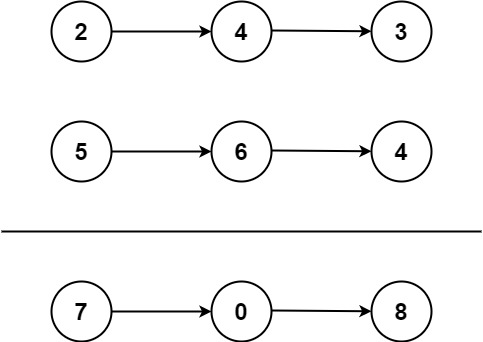
\includegraphics[width=0.6\textwidth]{img/addtwonumber1.jpg}
  \centering
\end{figure}

\begin{lstlisting}
Input: l1 = [2,4,3], l2 = [5,6,4]
Output: [7,0,8]
Explanation: 342 + 465 = 807.
\end{lstlisting}


\subsection*{Example 2:}

\begin{lstlisting}
Input: l1 = [0], l2 = [0]
Output: [0]
\end{lstlisting}


\subsection*{Example 3:}

\begin{lstlisting}
Input: l1 = [9,9,9,9,9,9,9], l2 = [9,9,9,9]
Output: [8,9,9,9,0,0,0,1]
\end{lstlisting}


\subsection*{Constraints:}

\begin{itemize}
  \item{The number of nodes in each linked list is in the range \code{[1, 100]}.}
  \item{\code{0 <= Node.val <= 9}}
  \item{It is guaranteed that the list represents a number that does not have leading zeros.}
\end{itemize}


\clearpage
